\chapter[Creation and Training of Spectral ViT]{Creation and Training of\newline Spectral ViT}
%Ensure that the chapter title fits on the header lines, but doesn't hyphenate on the chapter title page
\label{chap:methods}
% Methods to validate transformers (fake spectra), create training data (fake spectra), 
% train various models (V1.1, V1.2, V1.3, V2), to find optimal training for V2

In order to examine the effectiveness of the transformer architecture for supernovae
spectral classification, the following series of steps were taken. First, a custom transformer 
architecture was created based on the traditional ViT architecture \parencite{dosovitskiy2020}, 
and trained on a simple synthetic dataset to validate our approach. Next, a synthetic dataset 
using DESI spectra was created under a variety of preprocessing conditions. The previously 
created CNN and new transformer architectures were trained on the
preprocessed data. Finally, these training sessions were then used to determine 
the optimal training conditions for non-redshift corrected data. 

\section{Creation of Spectral ViT}\label{sec:SpecViT}
The Spectral ViT architecture was coded using the \texttt{PyTorch}
deep learning framework. The architecture is shown graphically in
Appendix~\ref{app:SpecViT}. The Spectral ViT is
composed of three main components: the pre-processor, the encoder, and the classifier. 

The pre-processing component is responsible for taking the 
input spectra extracted from the DESI CCDs and converting them into a series of 
vectors that the transformer can interpret. 
Consider a sample of $N$ spectra, each with $10000$ pixels corresponding to a bin containing a wavelength 
between $3600\AA$ and $9800\AA$. Each group is split into a set number of patches 
(approximately 100 pixels in length). Each patch is then 
linearly mapped via a fully connected network to a vector 4 times smaller than the patch size.
The sample is now a set of size $N\times100\times25$. 
A classification token of the same dimension as the patches 
is initialized with uniformly distributed random values between 0 and 1, and then concatenated to the beginning of each sample.
In order for the transformer to properly understand the positional relationship between each patch, an embedding 
is added to each patch. This embedding is a scalar function based on the size 
of the patch and is calculated as follows: 
\begin{equation}
    \text{Embedding}_{ij} = \begin{cases} \sin\left(\frac{i}{10000^{(j / \text{patch size})}}\right) & \text{if } j \text{ is even} \\
    \cos\left(\frac{i}{10000^{((j - 1) / \text{patch size})}}\right) & \text{if } j \text{ is odd}\end{cases},
\end{equation}
where $i$ is the patch index, $j$ is the index in the hidden dimension, and 
the patch size is the number of pixels defined in each patch \parencite{vaswani2017}. 
In a CNN, the positional relationship between each pixel is understood by the convolutional layers
and the pooling layers. However, without the positional embeddings, there is no difference between 
the first and last patch in the sample. The sinusoidal embeddings were chosen in 
alignment with the original transformer architecture \parencite{vaswani2017}, as well 
as providing a simple way to encode the positional information. A visual 
representation of the embeddings for the sample is shown in Fig.~\ref{fig:embedding}. Once the 
embeddings are added element-wise to the patches, the resulting tensor (of size $N\times101\times300$) is then passed through the encoder. 
\begin{figure}[t]
    \centering
    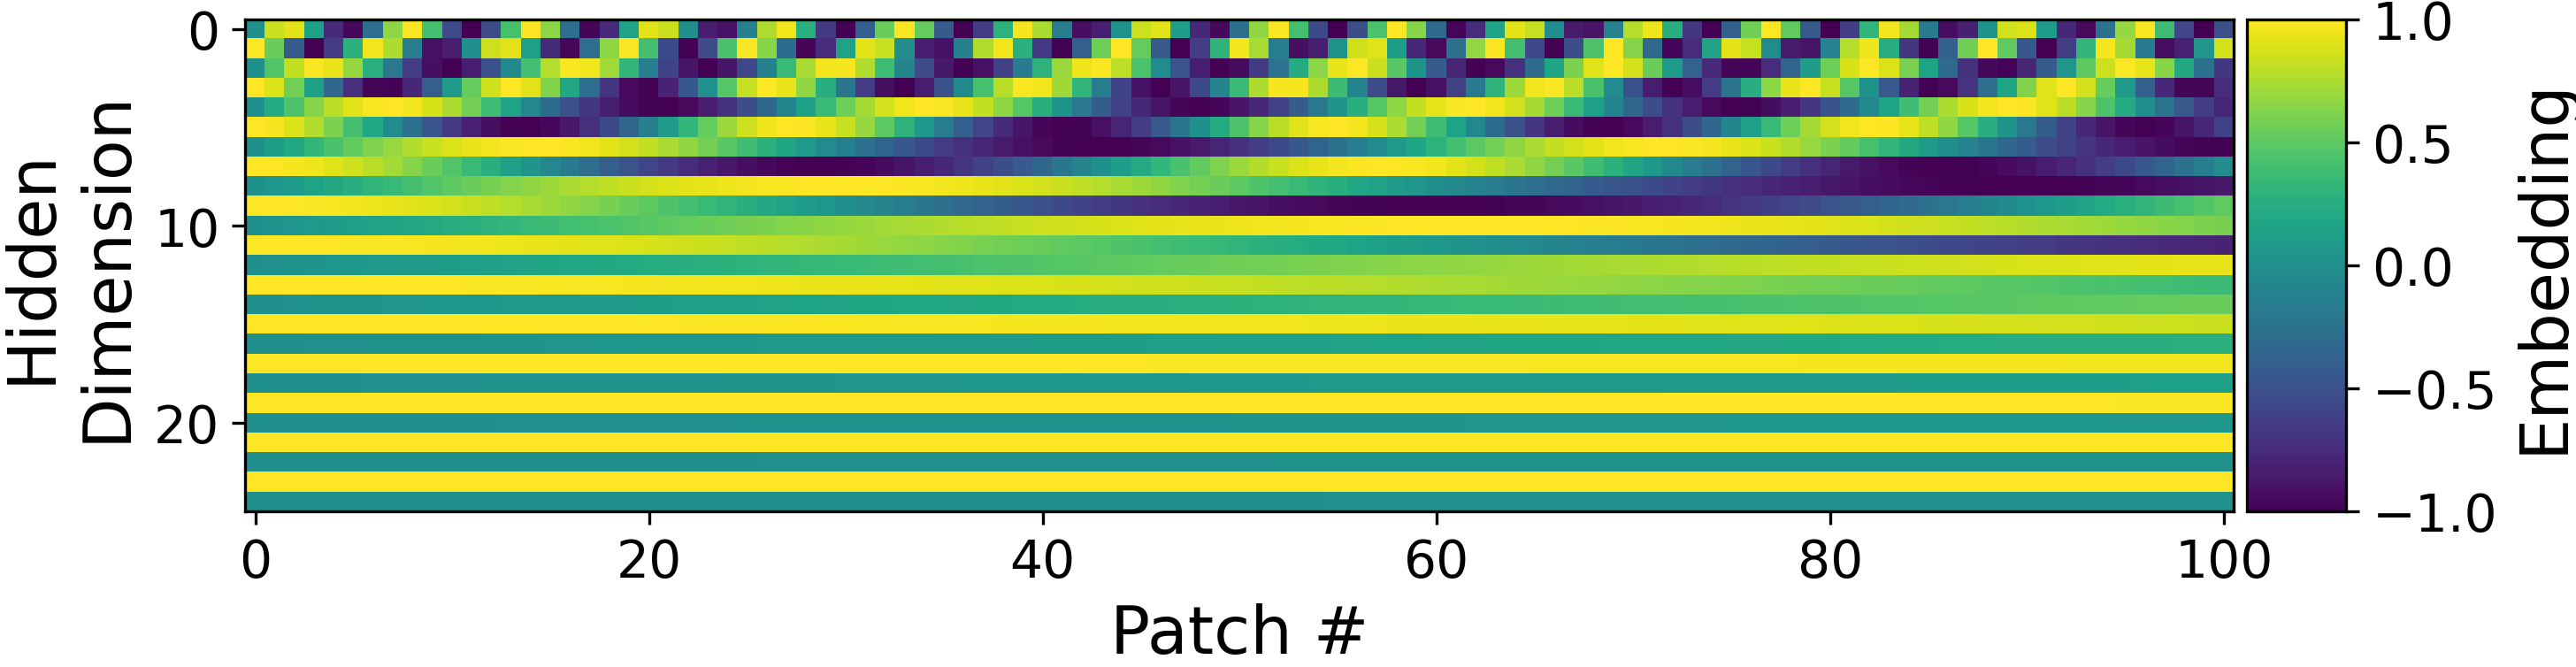
\includegraphics[width=\linewidth]{figures/embeddings_new.png}
    \caption{Visual representation of the embeddings for a sample of spectra. The x-axis represents the 
    index of the patch, the y-axis represents the index of the hidden dimension, and the color represents 
the value of the embedding.}
    \label{fig:embedding}
\end{figure}

The encoder is the main component of any ViT architecture, as it contains the 
multi-head attention and feed-forward layers. The encoder is composed of a user-defined number of
transformer blocks, each of which contains layer normalization, multi-head attention, another 
layer normalization, and finally a feed-forward layer. The multi-head attention layer 
used in this work is a scaled dot-product attention layer found in \textcite{vaswani2017}. Each patch 
is passed through three separate linear layers, each with a different set of weights, 
resulting in three sets of vectors: the query ($Q$), key ($K$), and value ($V$).
\begin{equation}
    \label{eq:mhsa}
    \text{Attention}(Q, K, V) = \text{softmax}\left(\frac{Q\cdot K^T}{\sqrt{d_k}}\right)\cdot V
\end{equation}
The dot-product between the query and key vectors is then calculated,
scaled by the square root of the dimensionality of the query vector, and then passed through a softmax function, 
defined as follows:
\begin{equation}
    \text{softmax}(x_i) = \frac{e^{x_i}}{\sum_{j=1}^N e^{x_j}}.
\end{equation}
The resulting attention weights are then multiplied by the value vectors (Equation~\ref{eq:mhsa}). 
This is simultaneously done for each head in the multi-head attention layer. Each result is then 
concatenated together, and then passed through a linear layer to reduce the dimensionality
to the size of the query vector. This resulting vector is then added
element-wise to the original patches, normalized, and then passed through a MLP, 
resulting in a tensor of size $N \times 101 \times 300$. This again is added element-wise to the original patches. 
Each step is repeated for a user-defined number of transformer blocks, resulting in a tensor of size
$N \times 101 \times 300$.

The final component of the Spectral ViT architecture is the classifier. The classifier
takes in only the first patch of each sample, which has been designated as the classification token.
The classification token is passed through a linear layer to reduce the dimensionality to the
number of classes, and then passed through a softmax function to produce a probability distribution
over the classes. Therefore, the resulting tensor is of size $N \times 1 \times 6$, for our 
6 classes of supernovae.

\subsection{Validation of Spectral ViT Architecture}
\label{ssec:validation}
After creating the Spectral ViT architecture, we tested our  ability to train it 
effectively. A synthetic dataset, consisting of a continuum with 
broad Gaussian peaks placed at predetermined locations. Certain combinations of 
peak locations were chosen to represent an arbitrary `class' of supernovae. These peaks, 
our synthetic emission lines, were given random amplitudes and widths, simulating  
variability, with a maximum allowed value. 
\textit{ % TODO: CORRECT THIS SENTANCE
This maximum allowed value was then used to add 
Gaussian noise to the signal: either 2 or 10 times the signal to simulate noisy ($S/N=2$),
or very good data ($S/N=10$).
}
Examples of the synthetic spectra with different continuum profiles 
are shown in Fig.~\ref{fig:synth_spectra}. 

These datasets with SNR=10 were trivially separable by a Spectral ViT architecture 
with two transformer blocks, two transformer heads, eight hidden layers, and a patch size of 16 (spectra were 1024 pixels long). 
An accuracy of 100\% on the testing set was achieved within 5 epochs of training (Figure~\ref{fig:snr10}). Trained on the same 
architecture, the data with SNR=2 was more difficult to separate, only achieving a 33.975\% test accuracy (Figure~\ref{fig:snr2}).


\begin{figure}
    \centering
    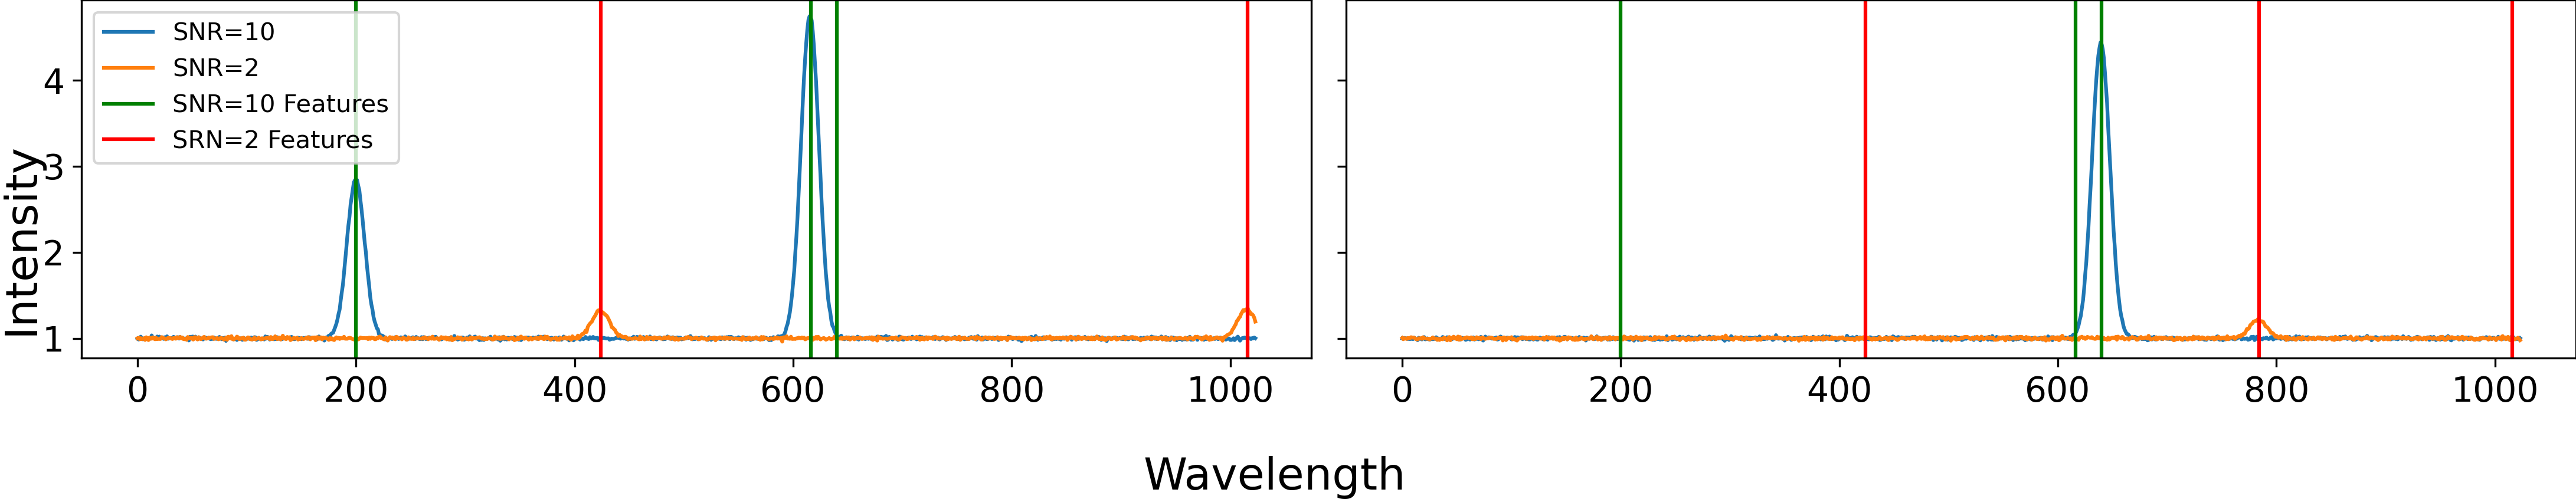
\includegraphics[width=\textwidth]{figures/synth_data_new.png}
    \caption{Synthetic spectra used to verify performance of SpectralViT. Red and green vertical lines represent features used to 
    seperate the data into disticnt classes for SNR=2 and SNR=10, respectively. Two classes are shown for each SNR.}
    \label{fig:synth_spectra}
\end{figure}

% Make into subcaptions
\begin{figure}[h]
    \centering
    \subfloat[\centering~SNR = 2\label{fig:snr2}]{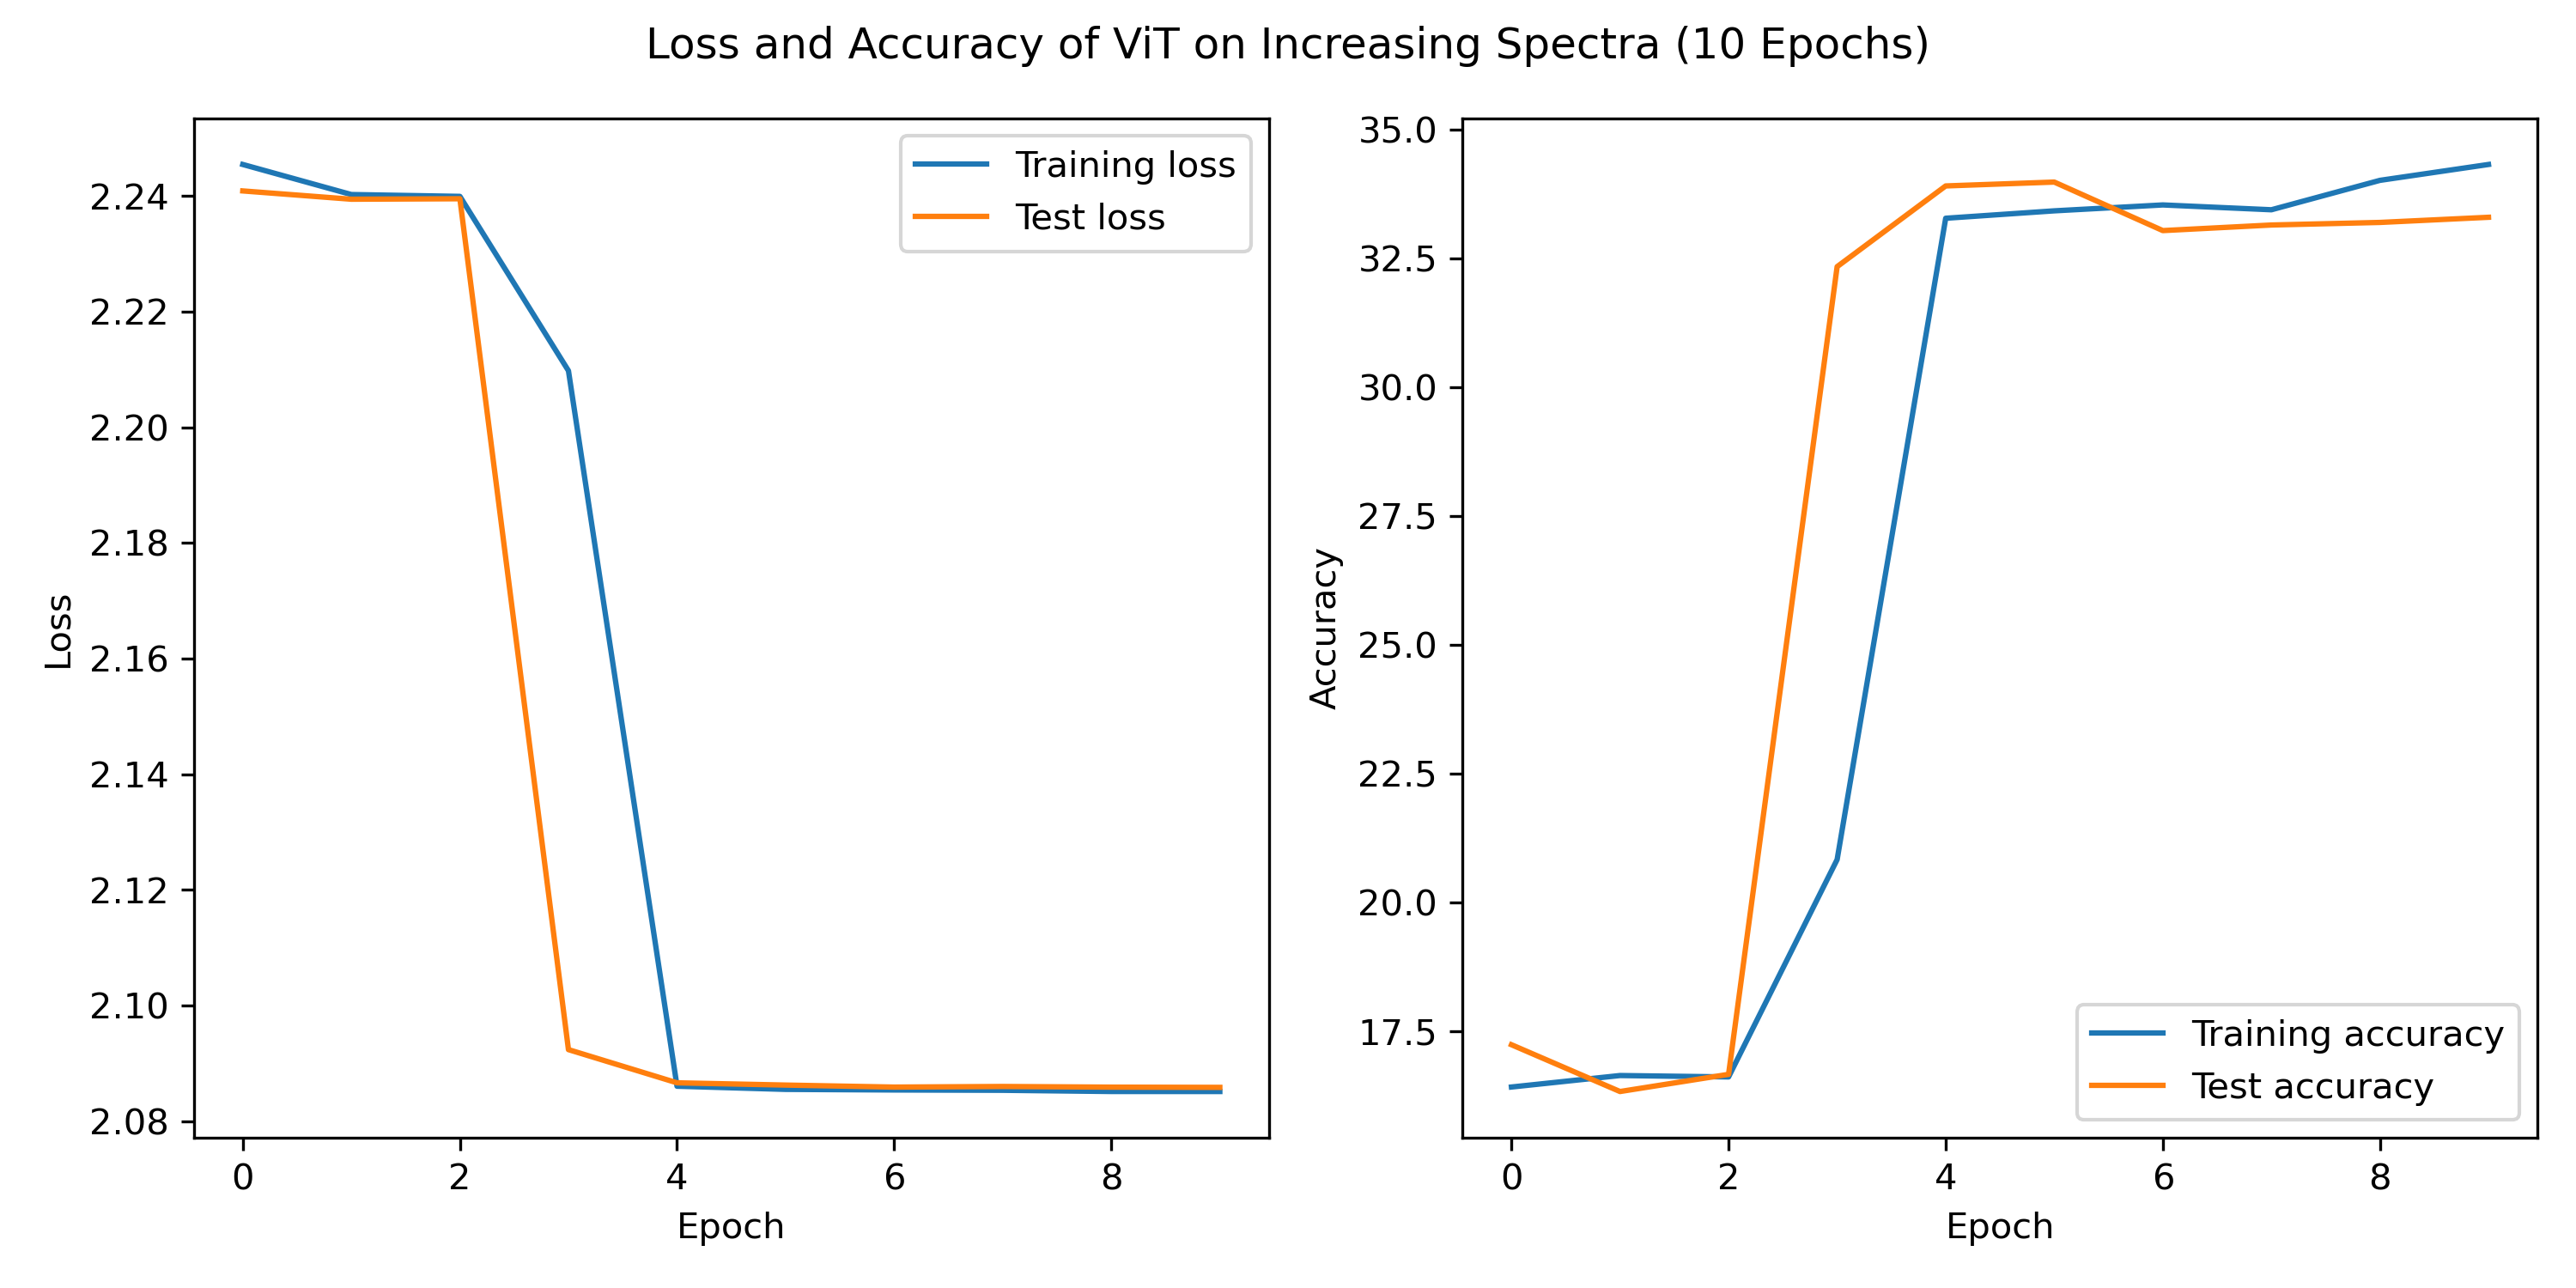
\includegraphics[width=10cm]{figures/pre_testing/SNR2_training_epoch.png}}
    \qquad
    \subfloat[\centering~SNR = 10\label{fig:snr10}]{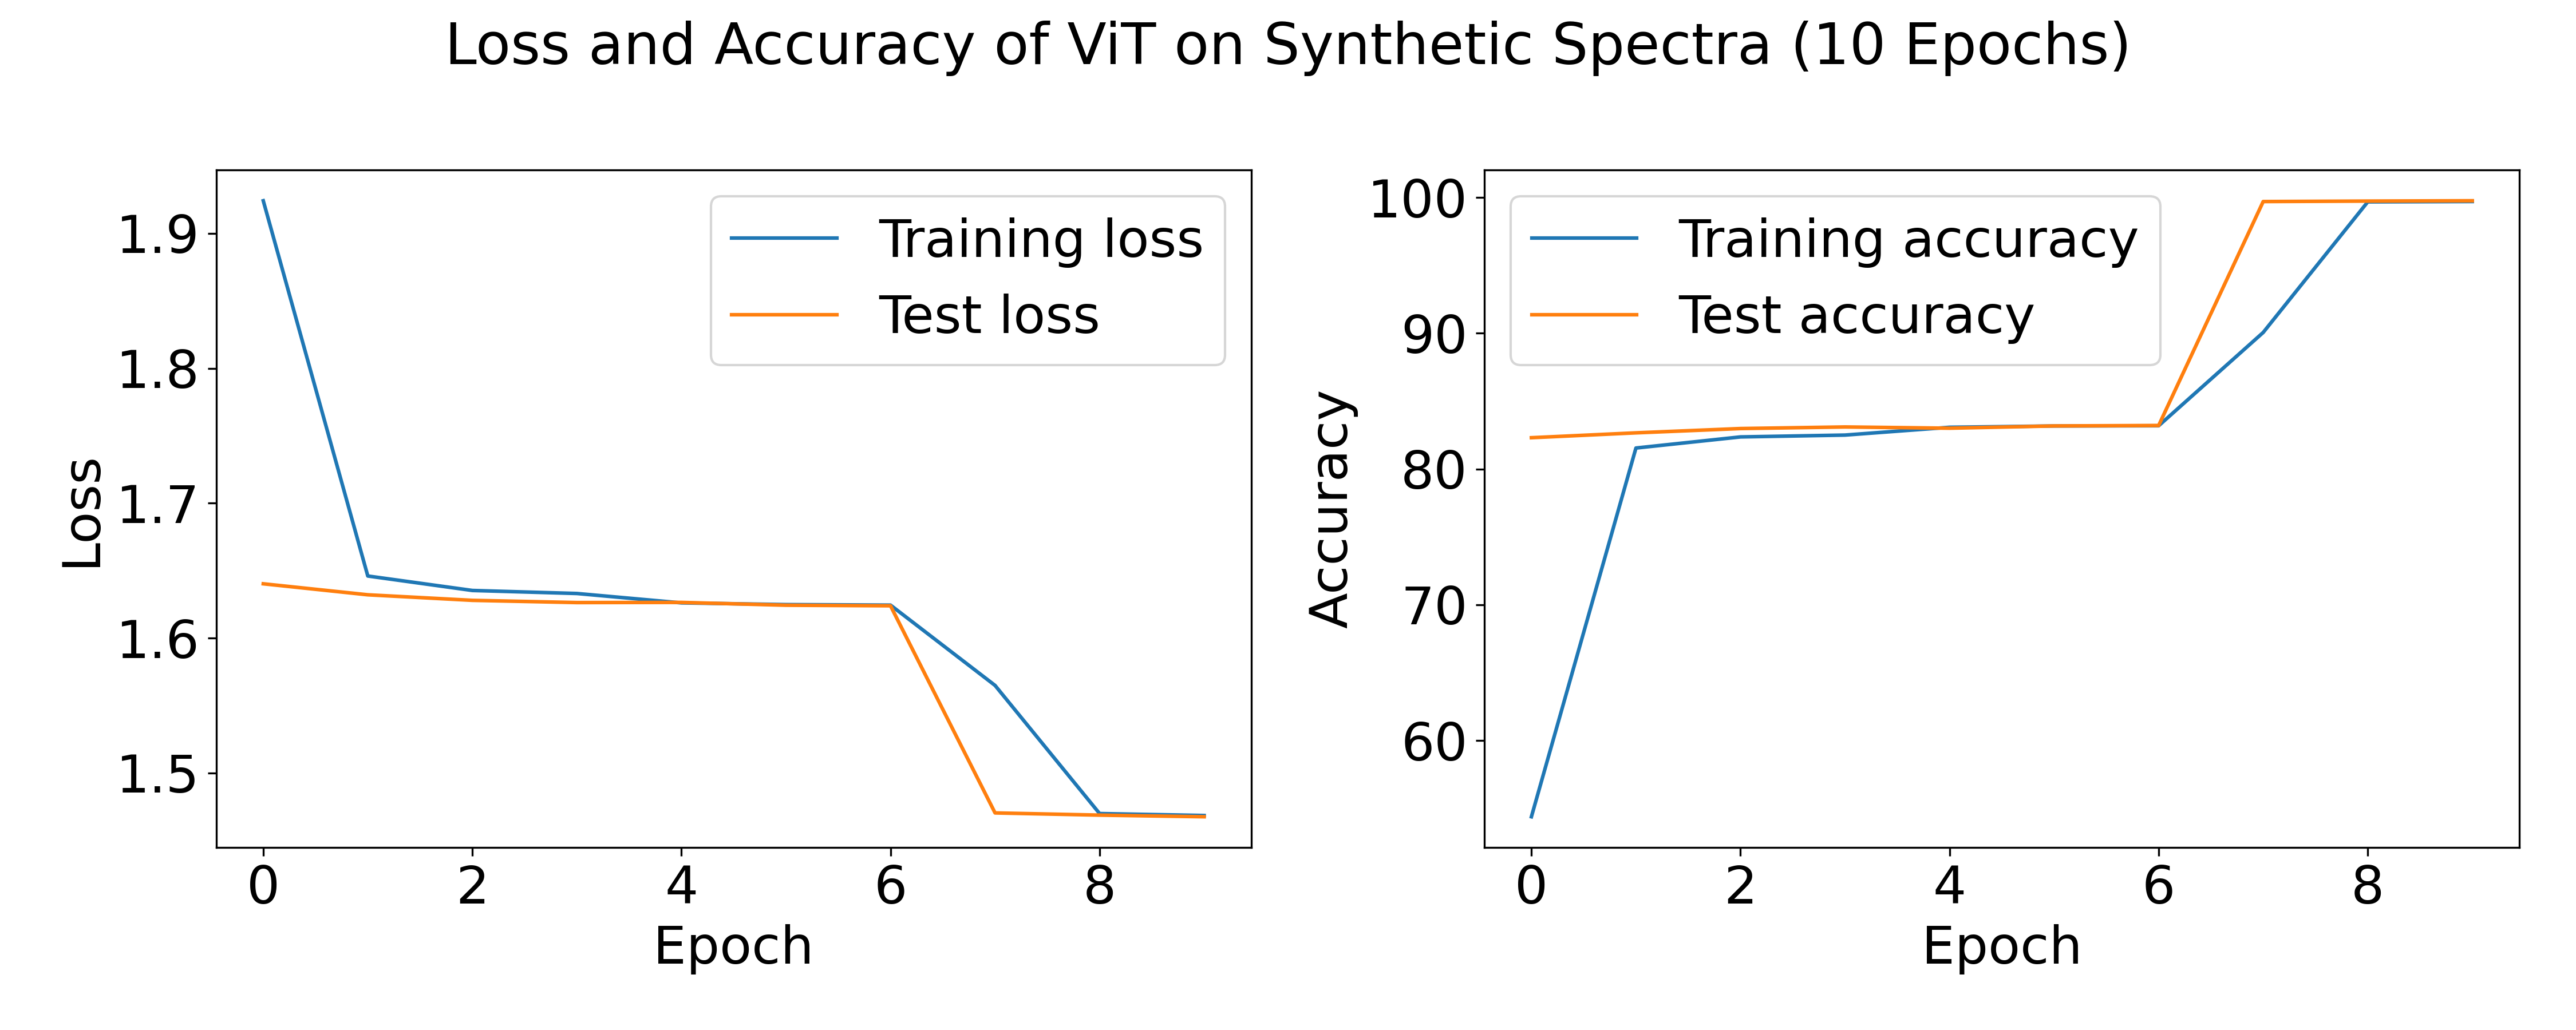
\includegraphics[width=10cm]{figures/pre_testing/SNR10_training_epoch.png}}
    \caption{Training of Spectral ViT on synthetic datasets. The model was able to reach 100\% accuracy on the test set of SNR=10 (top), 
    but failed to reach an accuracy of 50\% on the test set of SNR=2 (bottom).}
\label{fig:synth_spectra_training}
\end{figure}



\section{Creation of Synthetic DESI Spectra}
\label{sec:synth_data}
Once we demonstrated the Spectral ViT architecture was training effectively on simple synthetic data,
the architecture was trained on DESI data. In order to create a large enough training 
set, observed DESI spectra were used as a base to create synthetic spectra.

** Talk to BenZvi about what to put in this section / who to cite for all of the work **
** Couldn't find Eddies thesis online -- ask BenZvi fora copy ** 

\subsection{Pre-Processing of DESI Spectra}
\label{ssec:preprocess}
% All of preprocessing including z correction and downsampling 
Once the spectra was created and saved as DESI files, they needed to be 
extracted, preprocessed, split into training, testing, and validation sets, 
only then could they be saved, and used to train the Spectral ViT architecture.
The preprocessing method developed by ** Cite eddies paper **, and is split into 
3 main steps: redshift correction, rebinning / down sampling, and normalization. 

The reduced spectra, a table of best fit redshifts, and a set of fitting templates and 
coefficients are provided by the DESI pipeline in the form of a FITS file \parencite{Pence2010, Guy2023}.
The z correction step was used to move the spectra back into the rest frame using 
the best-fit redshift identified by the DESI pipeline. Next, all artifacts 
in the spectra (masks, bad pixels, etc.) were removed. The spectra were then re-binned
and downsampled to a user-defined resolution (default 3600). The spectra were then
normalized to redefine the maximum and minimum flux values to 1 and 0 respectively. Finally, for the 
CNN datasets, the spectra were split into a 2D array of equal height and width 
(i.e. for the spectra of length 3600, the array would have a shape of $60\times60$). 
After this, the spectra were split into training, testing and validation datasets that 
comprised 60\%, 20\%, and 20\% of the total dataset, respectively.
\begin{figure}[t]
    \centering
    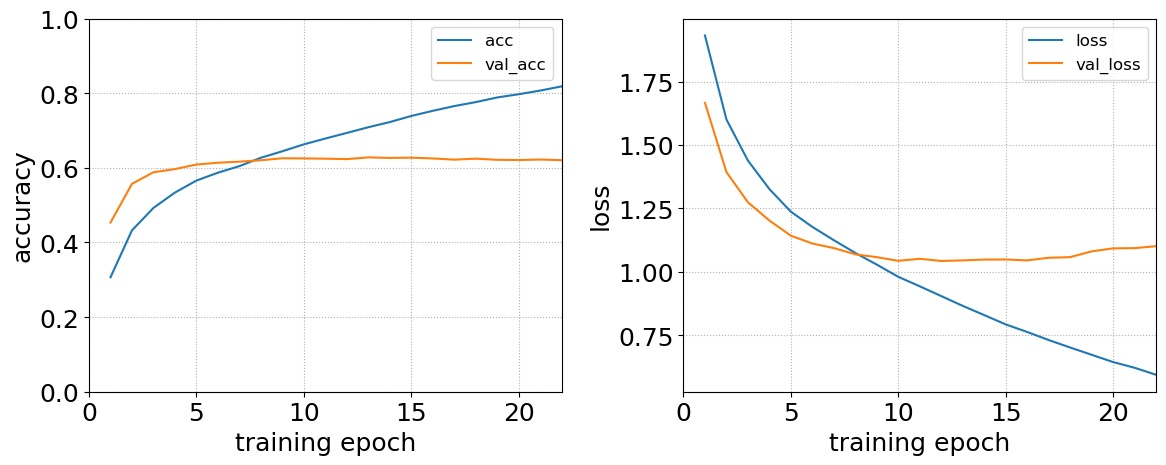
\includegraphics[width=.7\linewidth]{figures/cnn/cnn_training_history.jpg}
    \caption{Training of the CNN on synthetic DESI spectra.}
    \label{fig:cnn_training}
\end{figure}
\section{Training of Neural Networks}
\label{sec:training} 

\subsection{CNN Training}
\label{ssec:cnn_training}
The CNN architecture was developed by ** Cite eddies paper **, and has properties 
shown in Table~\ref{tab:cnn_architecture}.
This CNN was trained for a maximum of 50 epochs, with a batch size of 50, and 
non-variable hyperparameters (Table~\ref{tab:cnn_hyperparameters}). 
The timeline of the training of the CNN architecture is shown in Fig.~\ref{fig:cnn_training}.


\begin{table}[b]
    \small
    \centering
    \sffamily
    \begin{tabular}{lc}
	\toprule
    \textbf{Hyperparameter} & \textbf{Value} \\
    \midrule
    Learning Rate & 0.00004135238172950965 \\ 
    \midrule
    Regularization & 0.06 \\ 
    \midrule
    Dropout Rate & 0.40904759925886294\\
    \midrule
    Batch Size & 50 \\
    \bottomrule
\end{tabular}

    \caption{Hyperparameters of the CNN used to classify DESI spectra. CNN adapted 
    from \textcite{Sepeku2022}.}
    \label{tab:cnn_hyperparameters}
\end{table}

\subsection{Transformer Training}
\label{sec:transformer_training}
Two Spectral ViT architectures were trained on the synthetic DESI spectra.
The first architecture was smaller, while the second was larger. The properties 
of both are shown in Table~\ref{tab:t_hyper}. 
% \begin{table}
%     \small
%     \centering
%     \sffamily
%     \input{tables/transformer_small_hyperparameters.tex}
%     \caption{Hyperparameters of the smaller Spectral ViT architecture used to classify DESI spectra.}
%     \label{tab:t_hyper}
% \end{table}
Both were trained initially on spectra downsampled to 3600 bins. As shown in Figure~\ref{fig:vit1_training}, 
the smaller architecture was able to train effectively, reaching a test accuracy of 60.94\% after approximately 31 
epochs. The larger architecture was unable to train effectively, only reaching a test accuracy of around 26\% before 
overfitting, as shown in Figure~\ref{fig:vit1_big_training}. Therefore, the smaller architecture was chosen for further testing.

\begin{table}[t]
    \small
    \centering
    \sffamily
    \begin{tabular}{lcc}
	\toprule
    \textbf{Hyperparameter} & \textbf{Smaller Architecture} & \textbf{Larger Architecture} \\
    \midrule
    Learning Rate & 0.0001 & 0.01 \\ 
    \midrule
    Batch Size & 16 & 16 \\
    \midrule
    Blocks & 4 & 4 \\
    Heads & 5 & 12 \\
    Hidden Dimension & 25 & 72 \\
    \bottomrule
\end{tabular}

    \caption{Hyperparameters of the smaller and larger Spectral ViT architecture used to classify DESI spectra.}
    \label{tab:t_hyper}
\end{table}

\begin{figure}[b]
    \centering
    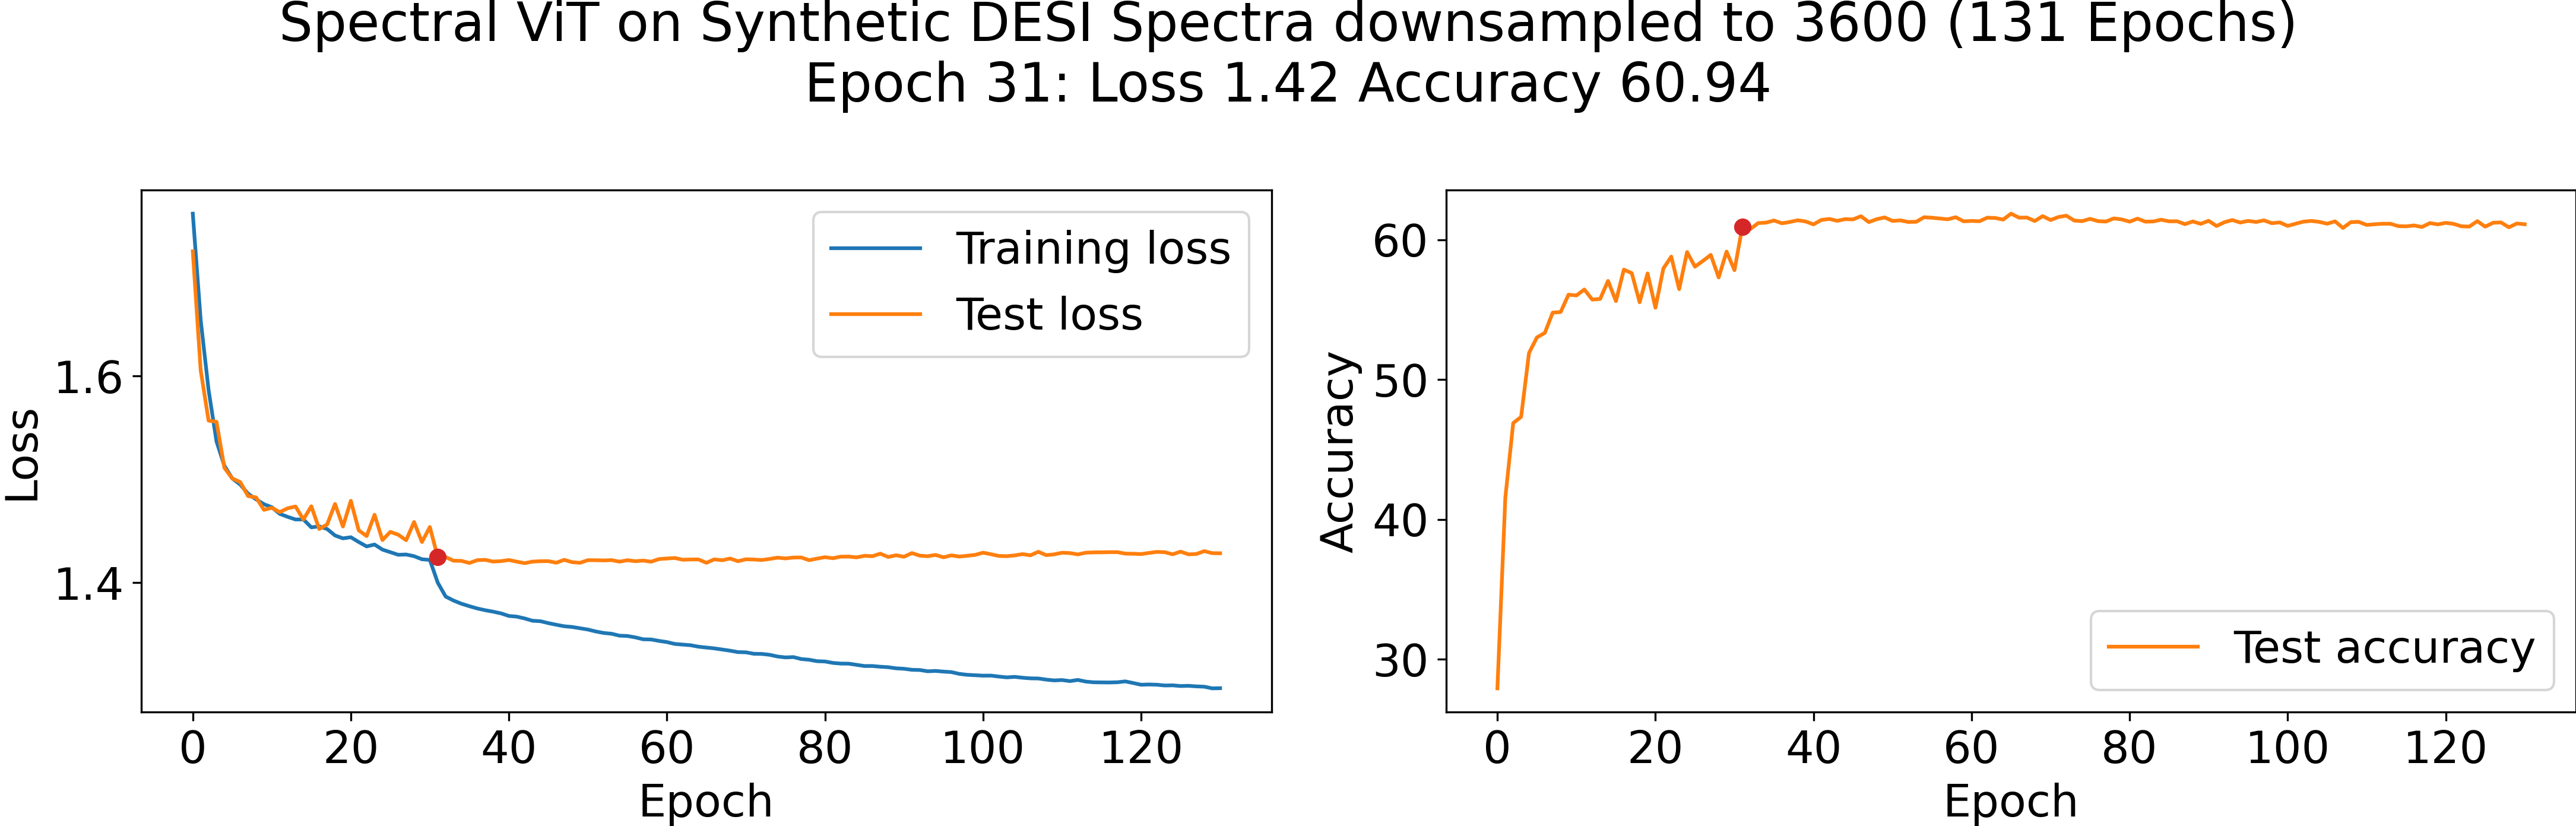
\includegraphics[width=.8\linewidth]{figures/v1_real/vit_model_V1_original_redotraining_new.png}
    \caption{Training of the small architecture on redshift-corrected spectra downsampled to 3600 bins. Over-fitting was determined to have occurred by Epoch 31.}
    \label{fig:vit1_training}
\end{figure}

\begin{figure}
    \centering
    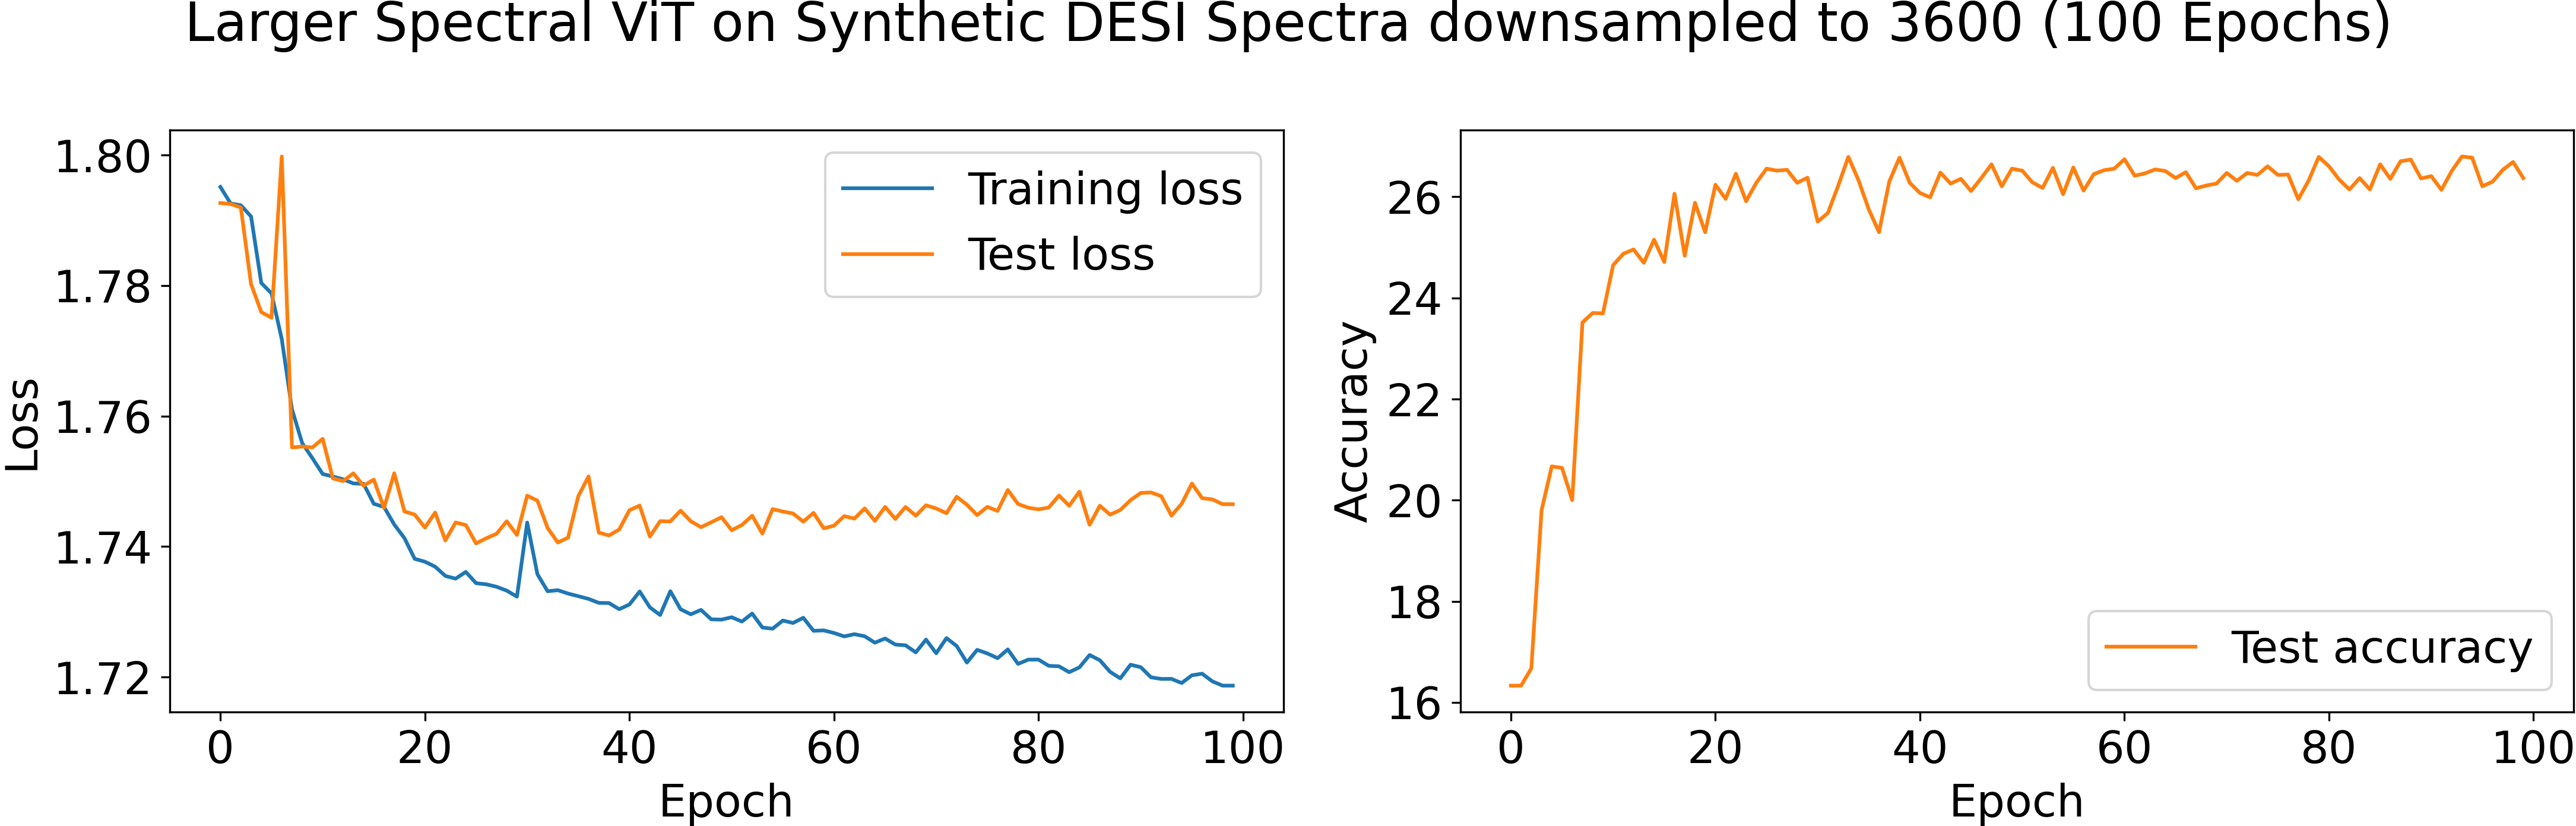
\includegraphics[width=.8\linewidth]{figures/v1_real/vit_model_V1_bigtraining_new.png}
    \caption{Training of the large architecture on Redshift-corrected spectra downsampled to 3600 bins. No convergence above random guessing was observed. }
    \label{fig:vit1_big_training}
\end{figure}

In addition, the smaller architecture was trained on spectra downsampled to 1800 and 900 bins to test 
its performance on spectra of varying resolution. As shown in Figure~\ref{fig:vit1.2_training} and Figure~\ref{fig:vit1.3_training},
neither variation was able to train as effectively as the original binning. 
\begin{figure}
    \centering
    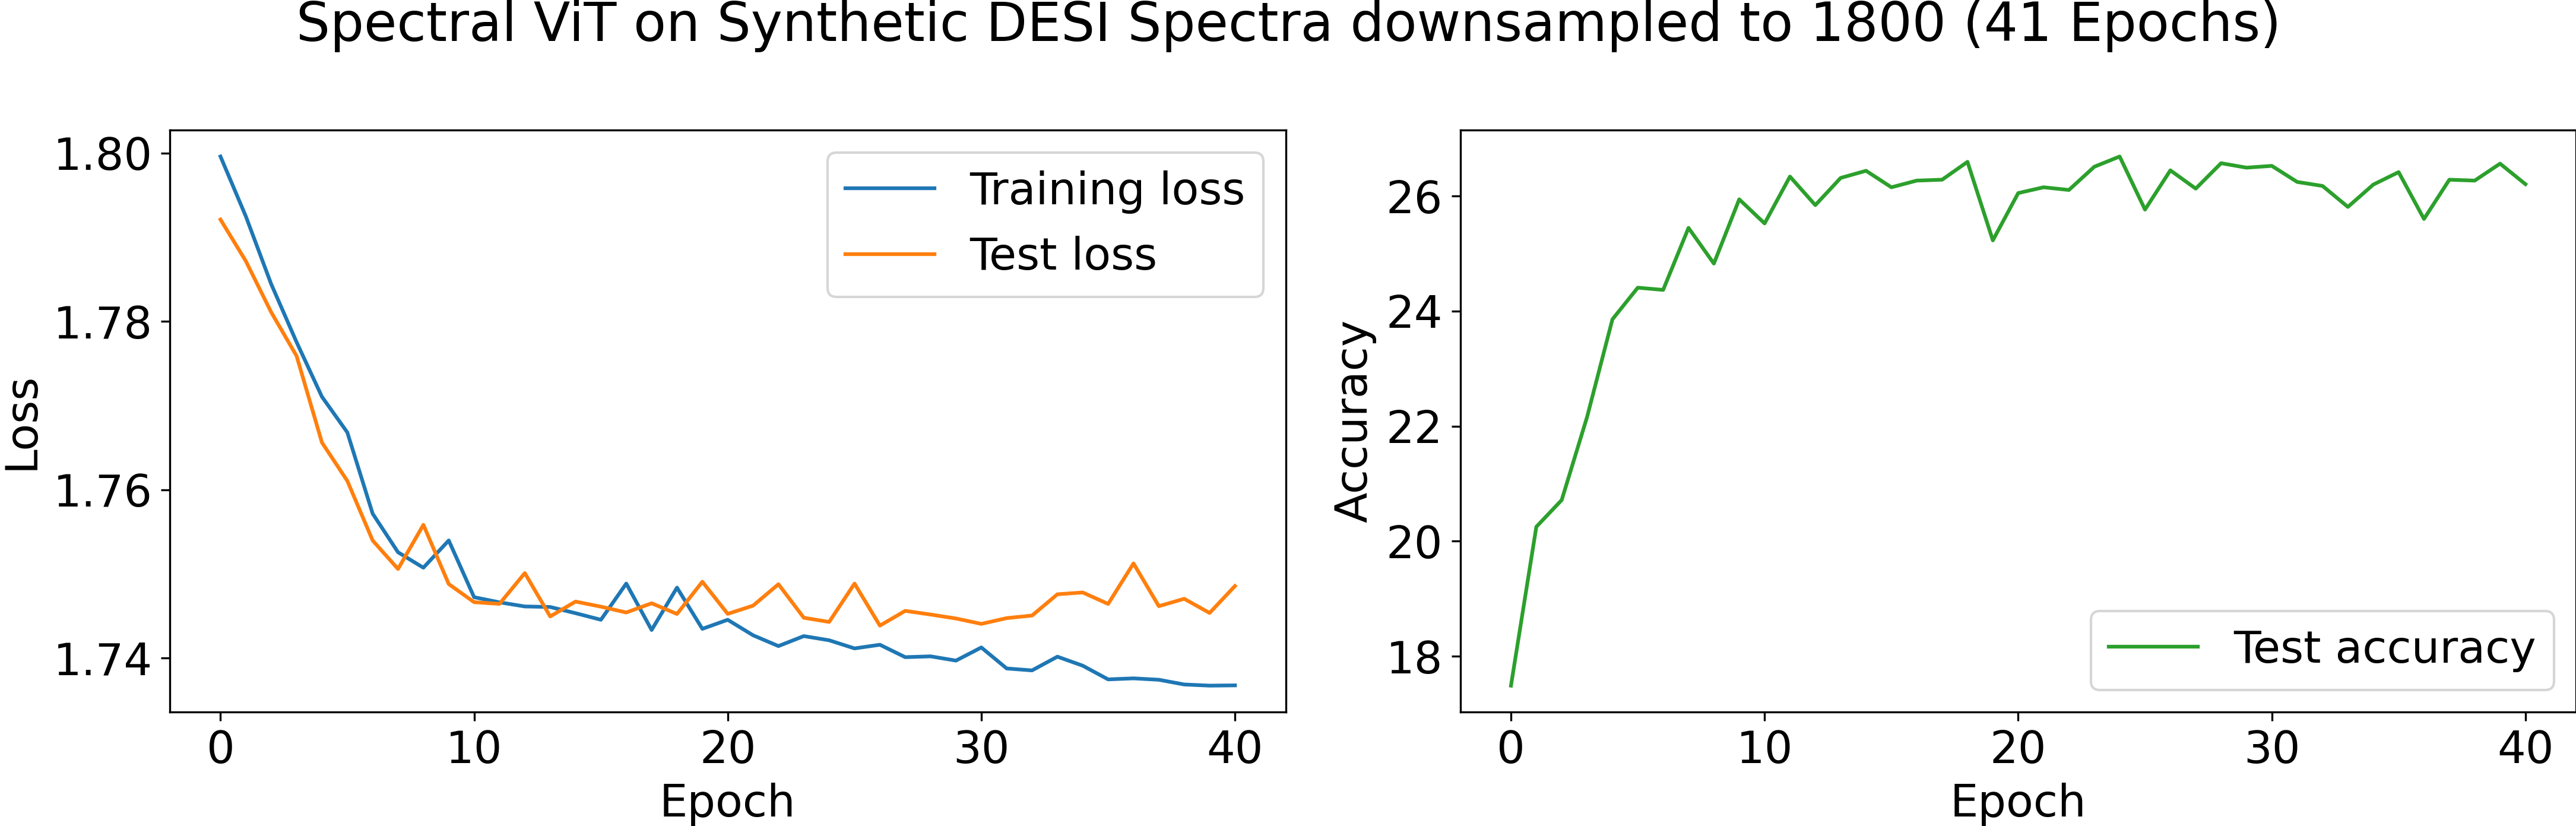
\includegraphics[width=.8\linewidth]{figures/vit_model_V1.2training_new.png}
    \caption{Training of the small architecture on Redshift-corrected spectra downsampled to 1800 bins. No convergence above random guessing was observed. }
    \label{fig:vit1.2_training}
\end{figure}

\begin{figure}
    \centering
    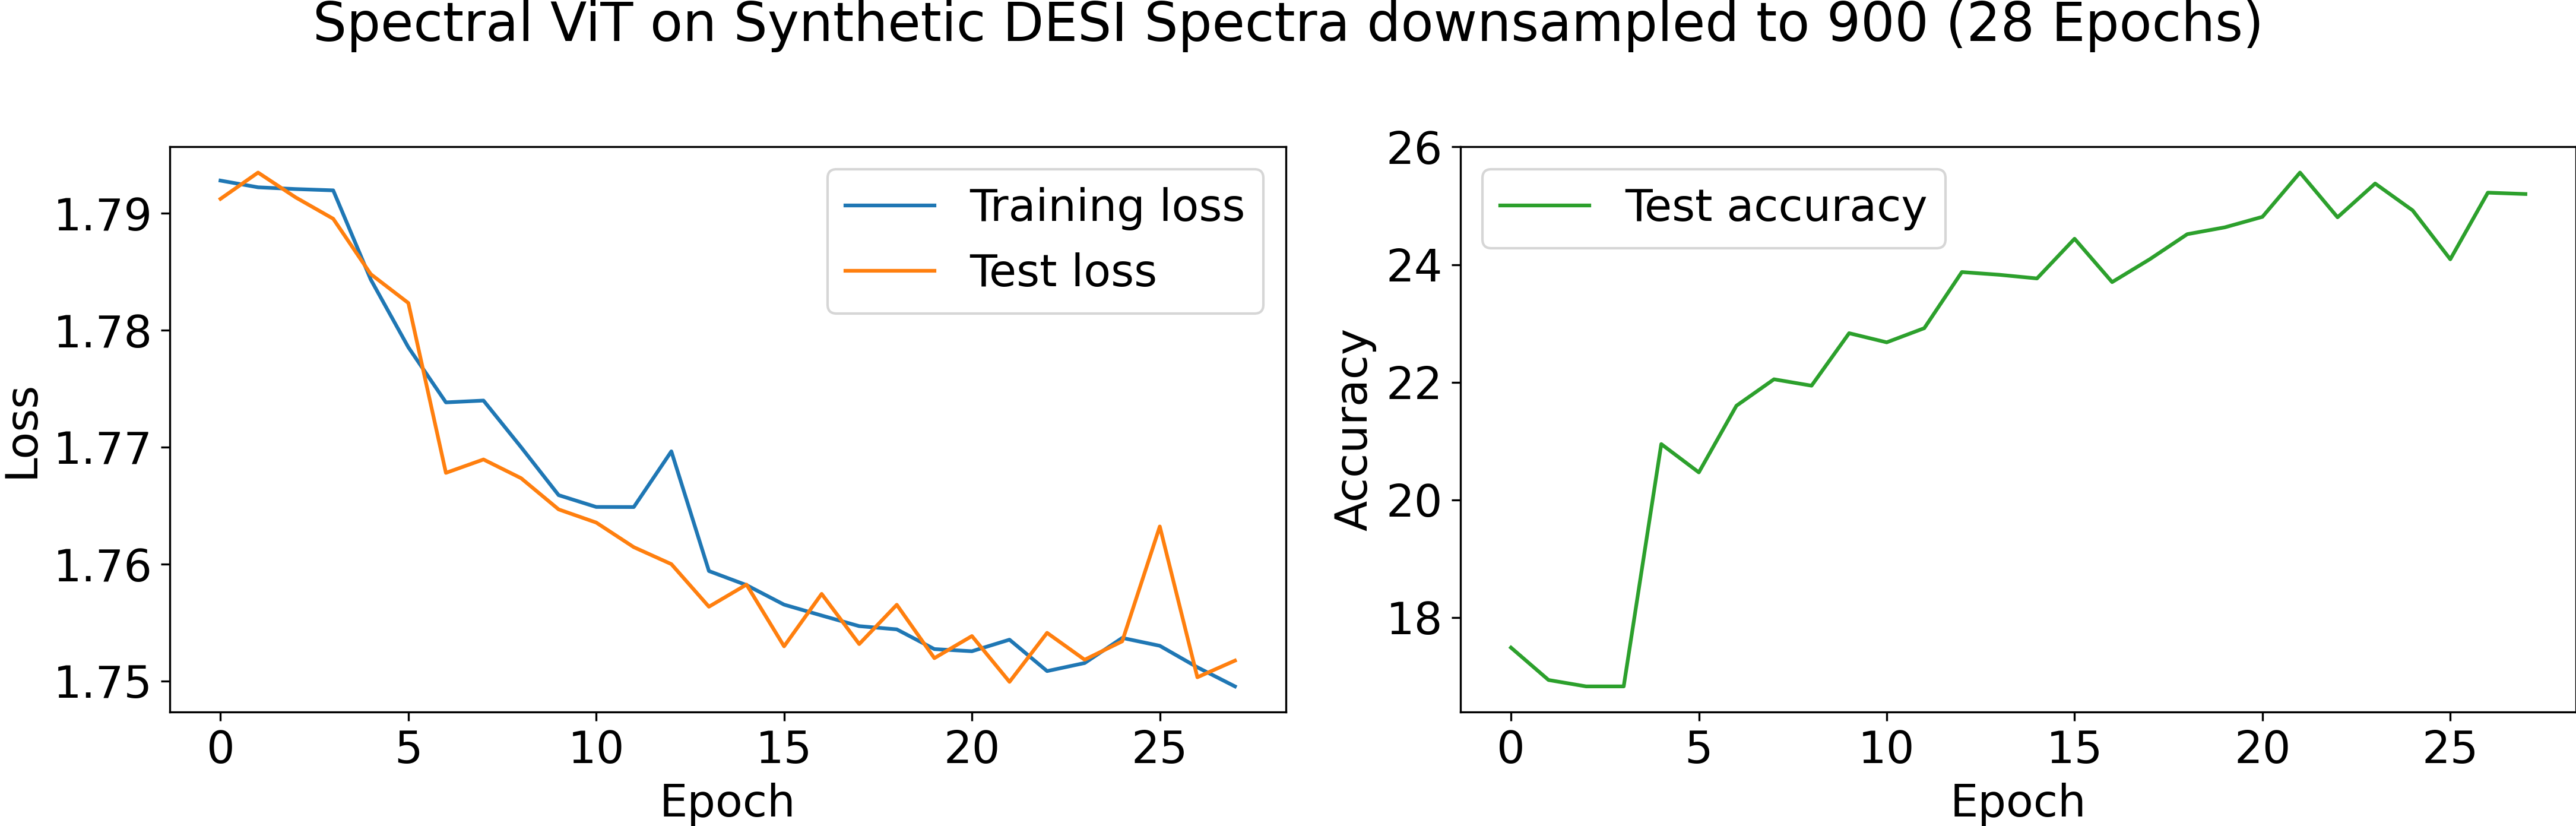
\includegraphics[width=.8\linewidth]{figures/vit_model_V1.3_muchsmallermodeltraining_new.png}
    \caption{Training of the small architecture on Redshift-corrected spectra downsampled to 900 bins. No convergence above random guessing was observed. }
    \label{fig:vit1.3_training}
\end{figure}

The smaller architecture, with a resolution of 3600 bins, was then trained on the non redshift-corrected spectra. 
As shown in Figure~\ref{fig:vit2_training}, the model was able to train effectively, reaching a test accuracy of 49.82\%. 


\begin{figure}
    \centering
    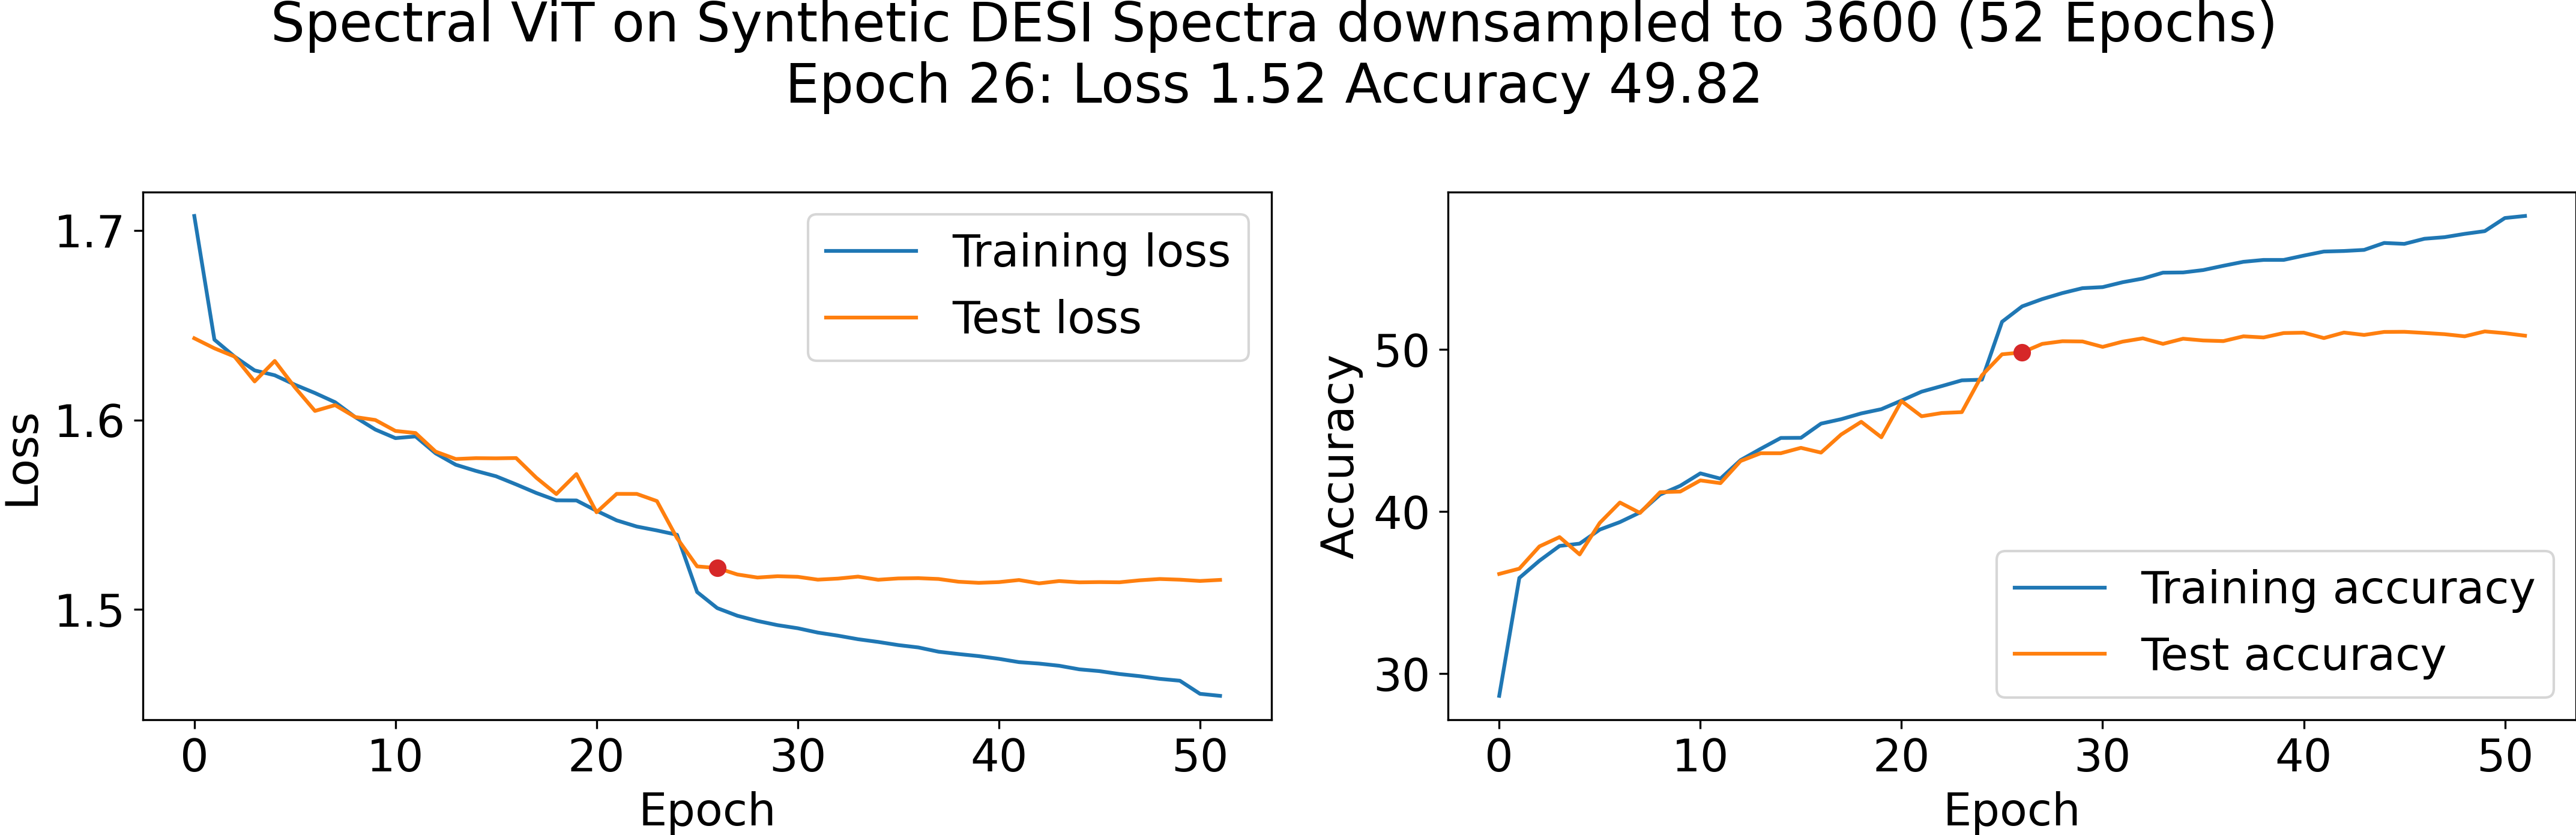
\includegraphics[width=.8\linewidth]{figures/v2_real/vit_model_V2training_new.png}
    \caption{Training of the small architecture on non Redshift-corrected data downsampled to 3600 bins. Over fitting was determined to have occurred by Epoch 26.}
    \label{fig:vit2_training}
\end{figure}
